% Options for packages loaded elsewhere
\PassOptionsToPackage{unicode}{hyperref}
\PassOptionsToPackage{hyphens}{url}
%
\documentclass[
]{article}
\usepackage{amsmath,amssymb}
\usepackage{iftex}
\ifPDFTeX
  \usepackage[T1]{fontenc}
  \usepackage[utf8]{inputenc}
  \usepackage{textcomp} % provide euro and other symbols
\else % if luatex or xetex
  \usepackage{unicode-math} % this also loads fontspec
  \defaultfontfeatures{Scale=MatchLowercase}
  \defaultfontfeatures[\rmfamily]{Ligatures=TeX,Scale=1}
\fi
\usepackage{lmodern}
\ifPDFTeX\else
  % xetex/luatex font selection
\fi
% Use upquote if available, for straight quotes in verbatim environments
\IfFileExists{upquote.sty}{\usepackage{upquote}}{}
\IfFileExists{microtype.sty}{% use microtype if available
  \usepackage[]{microtype}
  \UseMicrotypeSet[protrusion]{basicmath} % disable protrusion for tt fonts
}{}
\makeatletter
\@ifundefined{KOMAClassName}{% if non-KOMA class
  \IfFileExists{parskip.sty}{%
    \usepackage{parskip}
  }{% else
    \setlength{\parindent}{0pt}
    \setlength{\parskip}{6pt plus 2pt minus 1pt}}
}{% if KOMA class
  \KOMAoptions{parskip=half}}
\makeatother
\usepackage{xcolor}
\usepackage[margin=1in]{geometry}
\usepackage{color}
\usepackage{fancyvrb}
\newcommand{\VerbBar}{|}
\newcommand{\VERB}{\Verb[commandchars=\\\{\}]}
\DefineVerbatimEnvironment{Highlighting}{Verbatim}{commandchars=\\\{\}}
% Add ',fontsize=\small' for more characters per line
\usepackage{framed}
\definecolor{shadecolor}{RGB}{248,248,248}
\newenvironment{Shaded}{\begin{snugshade}}{\end{snugshade}}
\newcommand{\AlertTok}[1]{\textcolor[rgb]{0.94,0.16,0.16}{#1}}
\newcommand{\AnnotationTok}[1]{\textcolor[rgb]{0.56,0.35,0.01}{\textbf{\textit{#1}}}}
\newcommand{\AttributeTok}[1]{\textcolor[rgb]{0.13,0.29,0.53}{#1}}
\newcommand{\BaseNTok}[1]{\textcolor[rgb]{0.00,0.00,0.81}{#1}}
\newcommand{\BuiltInTok}[1]{#1}
\newcommand{\CharTok}[1]{\textcolor[rgb]{0.31,0.60,0.02}{#1}}
\newcommand{\CommentTok}[1]{\textcolor[rgb]{0.56,0.35,0.01}{\textit{#1}}}
\newcommand{\CommentVarTok}[1]{\textcolor[rgb]{0.56,0.35,0.01}{\textbf{\textit{#1}}}}
\newcommand{\ConstantTok}[1]{\textcolor[rgb]{0.56,0.35,0.01}{#1}}
\newcommand{\ControlFlowTok}[1]{\textcolor[rgb]{0.13,0.29,0.53}{\textbf{#1}}}
\newcommand{\DataTypeTok}[1]{\textcolor[rgb]{0.13,0.29,0.53}{#1}}
\newcommand{\DecValTok}[1]{\textcolor[rgb]{0.00,0.00,0.81}{#1}}
\newcommand{\DocumentationTok}[1]{\textcolor[rgb]{0.56,0.35,0.01}{\textbf{\textit{#1}}}}
\newcommand{\ErrorTok}[1]{\textcolor[rgb]{0.64,0.00,0.00}{\textbf{#1}}}
\newcommand{\ExtensionTok}[1]{#1}
\newcommand{\FloatTok}[1]{\textcolor[rgb]{0.00,0.00,0.81}{#1}}
\newcommand{\FunctionTok}[1]{\textcolor[rgb]{0.13,0.29,0.53}{\textbf{#1}}}
\newcommand{\ImportTok}[1]{#1}
\newcommand{\InformationTok}[1]{\textcolor[rgb]{0.56,0.35,0.01}{\textbf{\textit{#1}}}}
\newcommand{\KeywordTok}[1]{\textcolor[rgb]{0.13,0.29,0.53}{\textbf{#1}}}
\newcommand{\NormalTok}[1]{#1}
\newcommand{\OperatorTok}[1]{\textcolor[rgb]{0.81,0.36,0.00}{\textbf{#1}}}
\newcommand{\OtherTok}[1]{\textcolor[rgb]{0.56,0.35,0.01}{#1}}
\newcommand{\PreprocessorTok}[1]{\textcolor[rgb]{0.56,0.35,0.01}{\textit{#1}}}
\newcommand{\RegionMarkerTok}[1]{#1}
\newcommand{\SpecialCharTok}[1]{\textcolor[rgb]{0.81,0.36,0.00}{\textbf{#1}}}
\newcommand{\SpecialStringTok}[1]{\textcolor[rgb]{0.31,0.60,0.02}{#1}}
\newcommand{\StringTok}[1]{\textcolor[rgb]{0.31,0.60,0.02}{#1}}
\newcommand{\VariableTok}[1]{\textcolor[rgb]{0.00,0.00,0.00}{#1}}
\newcommand{\VerbatimStringTok}[1]{\textcolor[rgb]{0.31,0.60,0.02}{#1}}
\newcommand{\WarningTok}[1]{\textcolor[rgb]{0.56,0.35,0.01}{\textbf{\textit{#1}}}}
\usepackage{graphicx}
\makeatletter
\def\maxwidth{\ifdim\Gin@nat@width>\linewidth\linewidth\else\Gin@nat@width\fi}
\def\maxheight{\ifdim\Gin@nat@height>\textheight\textheight\else\Gin@nat@height\fi}
\makeatother
% Scale images if necessary, so that they will not overflow the page
% margins by default, and it is still possible to overwrite the defaults
% using explicit options in \includegraphics[width, height, ...]{}
\setkeys{Gin}{width=\maxwidth,height=\maxheight,keepaspectratio}
% Set default figure placement to htbp
\makeatletter
\def\fps@figure{htbp}
\makeatother
\setlength{\emergencystretch}{3em} % prevent overfull lines
\providecommand{\tightlist}{%
  \setlength{\itemsep}{0pt}\setlength{\parskip}{0pt}}
\setcounter{secnumdepth}{-\maxdimen} % remove section numbering
\usepackage{booktabs}
\usepackage{longtable}
\usepackage{array}
\usepackage{multirow}
\usepackage{wrapfig}
\usepackage{float}
\usepackage{colortbl}
\usepackage{pdflscape}
\usepackage{tabu}
\usepackage{threeparttable}
\usepackage{threeparttablex}
\usepackage[normalem]{ulem}
\usepackage{makecell}
\usepackage{xcolor}
\ifLuaTeX
  \usepackage{selnolig}  % disable illegal ligatures
\fi
\usepackage{bookmark}
\IfFileExists{xurl.sty}{\usepackage{xurl}}{} % add URL line breaks if available
\urlstyle{same}
\hypersetup{
  pdftitle={ Real Estate Pricing},
  pdfauthor={Victor Anton, Rodrigo Gonzalez \& Carlos Leon},
  hidelinks,
  pdfcreator={LaTeX via pandoc}}

\title{
\includegraphics[width=4in,height=\textheight]{images/LogoZugEstates.png}\\
Real Estate Pricing}
\author{Victor Anton, Rodrigo Gonzalez \& Carlos Leon}
\date{Machine Learning 1 - 05 June 2024}

\begin{document}
\maketitle

{
\setcounter{tocdepth}{3}
\tableofcontents
}
\section{Introduction}\label{introduction}

\textbf{Zug Estates (SWX: ZUGN)} focuses on developing, managing, and
marketing properties in the Zug region, Switzerland. As a company, they
prioritize centrally located sites for sustainable, multi-use
development.

Their portfolio is concentrated in \textbf{Zug} and \textbf{Risch
Rotkreuz}, featuring a mix of \textbf{residential}, \textbf{office},
\textbf{retail}, \textbf{hotel}, and \textbf{service spaces}. The
company aims for long-term property retention and development, driving
value creation through sustainable designs and active management.

\textbf{Zug Estates}, a major real estate player in Zug, Switzerland,
might be looking to invest in other parts of the country for several
reasons. Here's a comprehensive breakdown:

\begin{itemize}
\item
  \textbf{Risk Reduction:} By spreading their investments across
  different cantons (Swiss states), Zug Estates reduces the risk
  associated with a downturn in Zug's market.
\item
  \textbf{Saturated Market:} Zug market could be saturated, meaning
  there are limited opportunities for profitable investments. Expanding
  to other areas allows Zug Estates to tap into new markets with higher
  potential returns.
\item
  \textbf{Connecting the Landscape:} Zug Estates' investments might have
  a strategic element beyond just individual properties. They could be
  acquiring properties near transportation hubs or in developing
  commercial centers.
\item
  \textbf{Reputation and Knowledge:} Over time, Zug Estates has built a
  strong reputation for high-quality development and property management
  within Zug. Expanding to other cantons allows them to leverage this
  reputation. They can attract partnerships with local developers or win
  contracts for projects in new areas based on their proven track
  record. Essentially, they bring their successful model to other parts
  of Switzerland.
\item
  \textbf{Capitalizing on Demand:} Zug Estates might be strategically
  responding to broader market trends across Switzerland. Perhaps
  there's a growing demand for specific property types, like student
  housing or retirement communities, in certain regions.
\end{itemize}

We will focus on satisfying Zug Estates as a client looking to expand
their operations.

\subsection{Motivation and Goal}\label{motivation-and-goal}

\textbf{WP Carey}, a prominent \textbf{Real Estate Investment Trust
(REIT)} known for its diversified portfolio of commercial properties,
has recently announced its strategic decision to \textbf{exit the Swiss
market}. This move marks a significant shift in the company's investment
strategy, focusing more on markets where they see greater
\textbf{potential for growth and stability}. As part of this exit,
\textbf{WP Carey} has successfully negotiated the sale of its assets
located in central Switzerland to \textbf{Zug Estates}, a leading Swiss
real estate company with a strong presence in the Zug region.


\includegraphics[width=4in,height=\textheight]{images/wp carey.JPG}

The \textbf{assets sold} include a mix of \textbf{high-value commercial
properties}, \textbf{office buildings}, and \textbf{mixed-use
developments} that have been integral to \textbf{WP Carey's Swiss
portfolio}. This transaction allows \textbf{WP Carey} to reallocate
capital towards more lucrative opportunities in other markets, while Zug
Estates stands to benefit significantly from the acquisition. By
integrating these prime assets into their existing portfolio,
\textbf{Zug Estates} can enhance its market position and leverage the
strategic locations of these properties to \textbf{attract new tenants}
and \textbf{increase rental income}. This acquisition underscores
\textbf{Zug Estates} commitment to expanding its footprint in central
Switzerland and reinforces its reputation as a \textbf{key player} in
the \textbf{Swiss Real Estate market}.

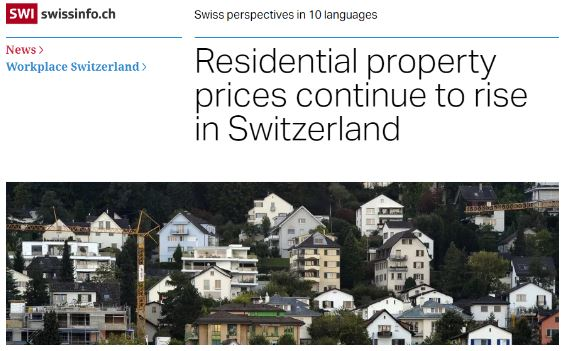
\includegraphics[width=10in,height=\textheight]{images/swissinfo.JPG}

Our team is deeply motivated to help Zug Estates by enhancing our
understanding of the real estate market in Central Switzerland. The
company's strategic approach has always attracted our attention, given
our recurring interest in real estate investment. We believe that the
future of Central Switzerland and Zug is bright, and this project
represents a unique opportunity to contribute to that growth. By
leveraging our collective expertise, we aim to provide valuable insights
that will help maximize the potential of these newly acquired assets.

For our analysis we will focus on residential real estate due to the
data limitations.

\textbf{Disclaimer:} \emph{This is a fictional situation created to
demonstrate students' ability to work with real datasets in situations
that could occur in the real world.}

\subsection{Dataset ``Homegate'' and ``Federal Statistic
Office''}\label{dataset-homegate-and-federal-statistic-office}

We used two data sources for this study:

First, \textbf{Homegate}, a \textbf{leading Swiss Real Estate platform},
has long been the go-to resource for individuals and businesses looking
to buy, sell, or rent properties in Switzerland. Known for its extensive
listings and user-friendly interface, \textbf{Homegate} provides
detailed information on a wide range of properties across the country.


\includegraphics[width=4in,height=\textheight]{images/homegate.JPG}

We have obtained a comprehensive dataset of properties listed on
Homegate, which will be invaluable for Zug Estates in evaluating these
assets and determining the best use for them. This dataset includes
detailed characteristics of the properties such as
\textbf{Property\_ID}, \textbf{FirstDay\_Online},
\textbf{LastDay\_Online}, \textbf{Type}, \textbf{Customer\_ID},
\textbf{Customer\_Segment}, \textbf{Category}, \textbf{Price\_Gross},
\textbf{Size\_m2}, \textbf{Canton}, \textbf{Nr\_rooms},
\textbf{Package\_ID}, and \textbf{Package\_Product}.

This private data has been obtained through legitimate channels and not
via scraping, ensuring their accuracy and reliability. With this rich
dataset, we will perform an in-depth analysis for Zug Estates to help
them understand market trends, property performance, and customer
preferences.

Second, \textbf{the Federal Statistical Office (FSO) in Switzerland}
offers a wealth of regional statistics that are essential for
understanding the diverse characteristics of the country's cantons.


\includegraphics[width=14in,height=\textheight]{images/federal.JPG}

Among these resources are the regional portraits and key figures, which
provide detailed portraits of each canton. These profiles include
crucial data points such as \textbf{Canton}, \textbf{Canton\_Name},
\textbf{Canton\_Capital}, \textbf{GDP\_2020\_21}, \textbf{GDP\_per},
Population, \textbf{Area\_km2}, \textbf{Density},
\textbf{Official\_Language\_1}, \textbf{Official\_Language\_2}, and
\textbf{Official\_Language\_3.} This information is invaluable for
stakeholders looking to gain insights into the economic, demographic,
and cultural landscape of Switzerland.

\subsection{Project Structure}\label{project-structure}

In order to offer the best insights into the data at hand, we structured
this project to work in a way that will help us first break down
different views on the data, and then work on gathering and creating
interesting conclusions for the stakeholders. We began with the
exploratory analysis, then brought in each of our models in order of
complexity, specifying each one's purpose as well as their conclusions.

We also realize that, when looking at the same data with different
models, points of view, and targets, the behavior perceived may differ
significantly. For this reason, we added a section for each model
explaining what our findings were and how they mean, and interpreting
them in a way that is digestible for readers.

Our intention overall was to find as much insight from available data to
help Zug Estates make the best decisions for their financial future,
proving how invaluable these tools can be. Fortunately, we were able to
make several conclusions that can be of great benefit for ZE, and have
gathered knowledge and tools that can most certainly aid in the future.

\subsection{Navigating the Report: Understanding the Hidden R
Code}\label{navigating-the-report-understanding-the-hidden-r-code}

This report is based on R code that was used to explore, train, and test
various models on the data. To maintain a clean and accessible format,
much of this code is hidden within the document.

However, upon request, the code can be made visible for thorough review.
This feature not only helps ensure the reproducibility of our analysis
but also facilitates ease of reading.

\section{Data Preparation}\label{data-preparation}

Before proceeding to the exploratory graphical analysis, this chapter
provides a brief overview of how the dataset was loaded and prepared.

\subsection{Libraries}\label{libraries}

In this report the following libraries are used.

\emph{Click to see all libraries}

\begin{Shaded}
\begin{Highlighting}[]
\CommentTok{\# used libraries}
\FunctionTok{library}\NormalTok{(readr)}
\FunctionTok{library}\NormalTok{(ggplot2)}
\FunctionTok{library}\NormalTok{(stringr)}
\FunctionTok{library}\NormalTok{(dplyr)}
\FunctionTok{library}\NormalTok{(readxl)}
\FunctionTok{library}\NormalTok{(openxlsx)}
\FunctionTok{library}\NormalTok{(lubridate)}
\FunctionTok{library}\NormalTok{(readxl)}
\FunctionTok{library}\NormalTok{(neuralnet)}
\FunctionTok{library}\NormalTok{(caret)}
\FunctionTok{library}\NormalTok{(e1071)}
\FunctionTok{library}\NormalTok{(gridExtra)}
\FunctionTok{library}\NormalTok{(mgcv)}
\FunctionTok{library}\NormalTok{(pROC)}
\FunctionTok{library}\NormalTok{(reshape2)}
\FunctionTok{library}\NormalTok{(tidyr)}
\FunctionTok{library}\NormalTok{(kableExtra)}
\FunctionTok{library}\NormalTok{(splines)}
\end{Highlighting}
\end{Shaded}

\section{Exploratory Data Analysis}\label{exploratory-data-analysis}

This chapter thoroughly explores the dataset, with a specific focus on
the main variable of interest: \textbf{rental prices}. Our primary goal
is to develop predictive models for rental prices of both apartments and
houses.

\subsection{Data Preparation and Preliminary
Analysis}\label{data-preparation-and-preliminary-analysis}

Before embarking on our data analysis journey, it was essential to
prepare our data, here the step by step:

\begin{itemize}
\item
  \textbf{Data Import and Merging:} The first step was to import our two
  datasets, named \textbf{``df\_kanton''} (information on the Swiss
  cantons) and \textbf{``df\_homegate''} (property characteristics
  including prices, size, number of rooms, etc). In order to work with
  one dataset, we merged the two datasets based on the
  \textbf{``Canton''} column into a new data frame.
\item
  \textbf{Data Filtering:} Some data points were not suitable for our
  intended use case because our focus is on houses and apartments. Other
  irrelevant property types were filtered out. Furthermore, we
  determined that analyzing the entire Swiss market was irrelevant for
  our purposes. Therefore, we limited our analysis to \textbf{Central
  Switzerland (Aargau (AG), Luzern (LU), Zurich (ZH)} and \textbf{Zug
  (ZG))} to maintain relevance and homogeneity.
\item
  \textbf{Preliminary Data Cleaning:} Before of cleaning the whole
  dataset we performed visualizations to identify and focus on
  interesting features.
\item
  \textbf{Data cleaning and preparation:}

  \begin{itemize}
  \item
    \textbf{Missing value handling:} Removed rows with missing values in
    key columns.
  \item
    \textbf{Feature engineering:} Created a new column
    \textbf{``Days\_Difference''} to capture the time difference between
    two date columns.
  \item
    \textbf{One-Hot Encoding:} Applied to categorical variables for
    better compatibility with machine learning models.
  \item
    \textbf{Label encoding:} Converted categorical variables to
    numerical representations.
  \end{itemize}
\end{itemize}

In summary, these steps prepared the data for further analysis and
modelling by cleaning it, handling missing values, and encoding
categorical variables, which are essential steps in data pre-processing
for machine learning tasks.

The dataset for our Exploratory Data Analysis includes the following
columns.

\emph{Click to see all column names}

\begin{verbatim}
##  [1] "Canton"              "Property_ID"         "FirstDay_Online"    
##  [4] "LastDay_Online"      "Type"                "Customer_ID"        
##  [7] "Customer_Segment"    "Category"            "Price_Gross"        
## [10] "Size_m2"             "Nr_rooms"            "Package_ID"         
## [13] "Package_Product"     "Canton_Name"         "Canton_Capital"     
## [16] "GDP_2020_21"         "GDP_per"             "Population"         
## [19] "Area_km2"            "Density"             "Official_Language_1"
## [22] "Official_Language_2" "Official_Language_3"
\end{verbatim}

Finally, the dataset for our Modeling includes the following columns.

\emph{Click to see all column names}

\begin{verbatim}
##  [1] "Canton_num"           "Days_Difference"      "Customer_Segment_num"
##  [4] "Category_num"         "Nr_rooms"             "Package_Product_num" 
##  [7] "GDP_2020_21"          "GDP_per"              "Population"          
## [10] "Area_km2"             "Density"              "Size_m2"             
## [13] "Price_Gross"
\end{verbatim}

\subsection{Data Visualization}\label{data-visualization}

\subsubsection{Properties per Canton}\label{properties-per-canton}

This bar chart shows the distribution of properties across different
cantons in Switzerland. Zurich (ZH) has the highest number of properties
listed, followed by Vaud (VD) and Aargau (AG), highlighting regional
differences in property availability.

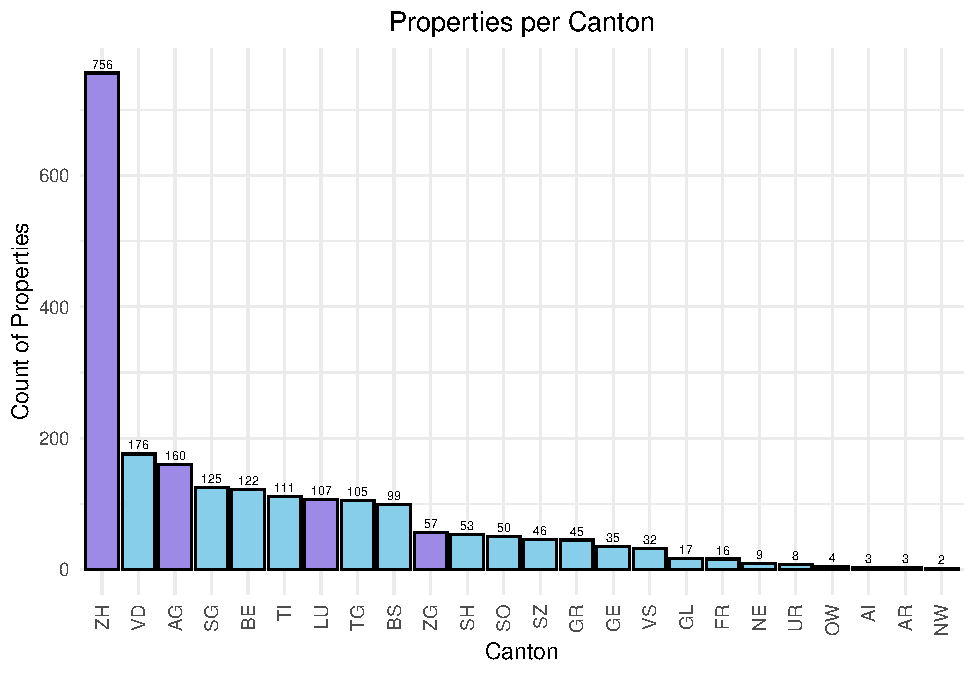
\includegraphics{2024_groupXX_report_files/figure-latex/Properties per Canton-1.pdf}

\subsubsection{Average Rental Price per
Canton}\label{average-rental-price-per-canton}

The visualizations compare average rental prices across Swiss cantons,
with the first chart showing the top ten cantons and highlighting the
exceptionally high average rental price in Ticino compared to others.

The second chart focuses on our study cantons of Zurich, Lucerne, Aargau
and Zug, illustrating more typical, affordable rental prices below CHF
2,000.

These charts highlight the significant regional differences in rental
costs within Switzerland, which is useful for market analysis,
investment decisions and policy formulation.

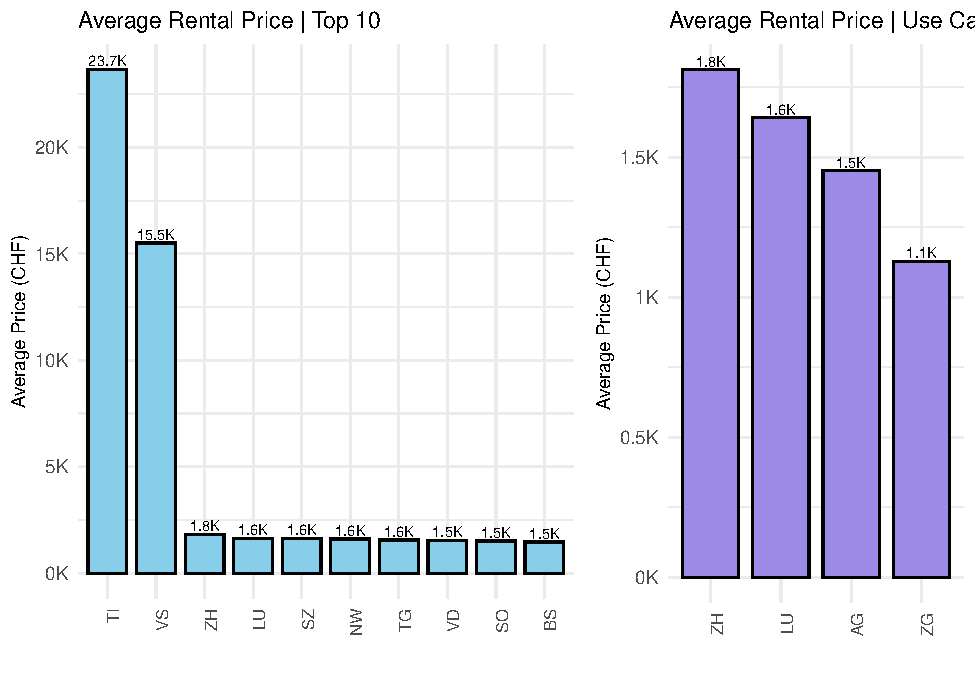
\includegraphics{2024_groupXX_report_files/figure-latex/unnamed-chunk-1-1.pdf}

\subsubsection{Differences in rental prices between different customer
segment}\label{differences-in-rental-prices-between-different-customer-segment}

The box plot compare the gross rental prices between private and
professional customer segments. Prices for private customers are
generally lower and less varied than those for professionals, indicating
a potential market segmentation by rental price.

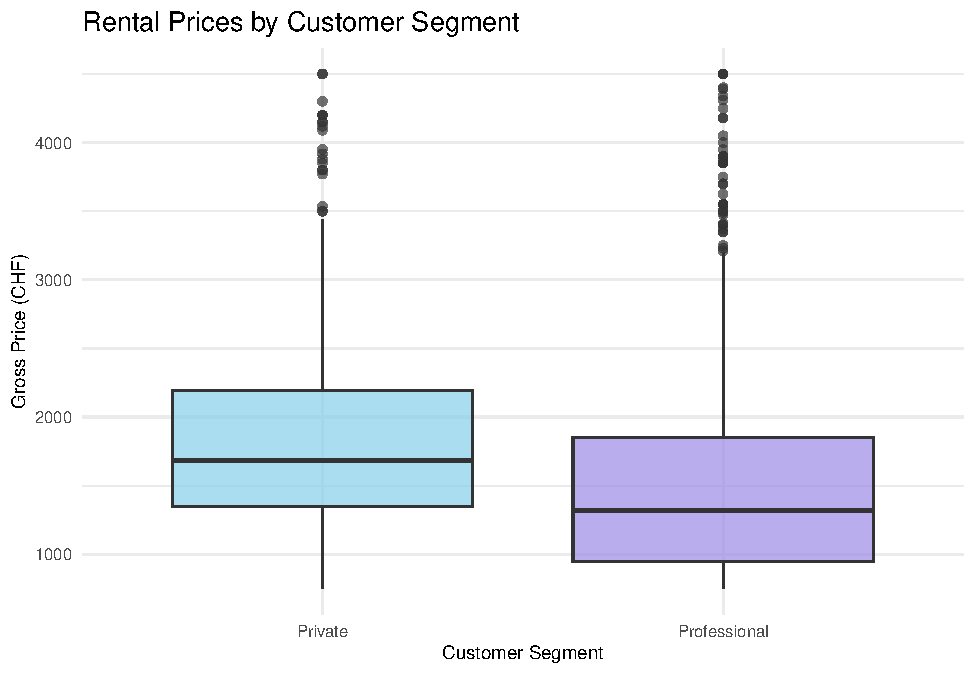
\includegraphics{2024_groupXX_report_files/figure-latex/Differences in rental prices between different customer segment-1.pdf}

\subsubsection{Influence of Property Size on Rental
Price}\label{influence-of-property-size-on-rental-price}

\begin{itemize}
\tightlist
\item
  \textbf{Correlation Between Property Size and Rental Price}
\end{itemize}

The scatter plot illustrates the correlation between property size and
rental price across Swiss cantons. The linear trend line shows a
positive correlation, indicating that as property size increases, the
gross rental price also tends to increase.

This trend is consistent across both the highlighted and other cantons,
suggesting that property size is a significant factor in determining
rental prices across the regions analyzed. The distinction between the
canton groups helps to visually assess whether there are any noticeable
differences in price trends based on location, which appear to be
relatively uniform across the board.

\begin{itemize}
\tightlist
\item
  \textbf{Distribution of Property Size}
\end{itemize}

This histogram highlights that the majority of properties fall within
smaller size brackets, with a steep drop-off as property size increases.
This distribution suggests that smaller properties are more common in
the market.

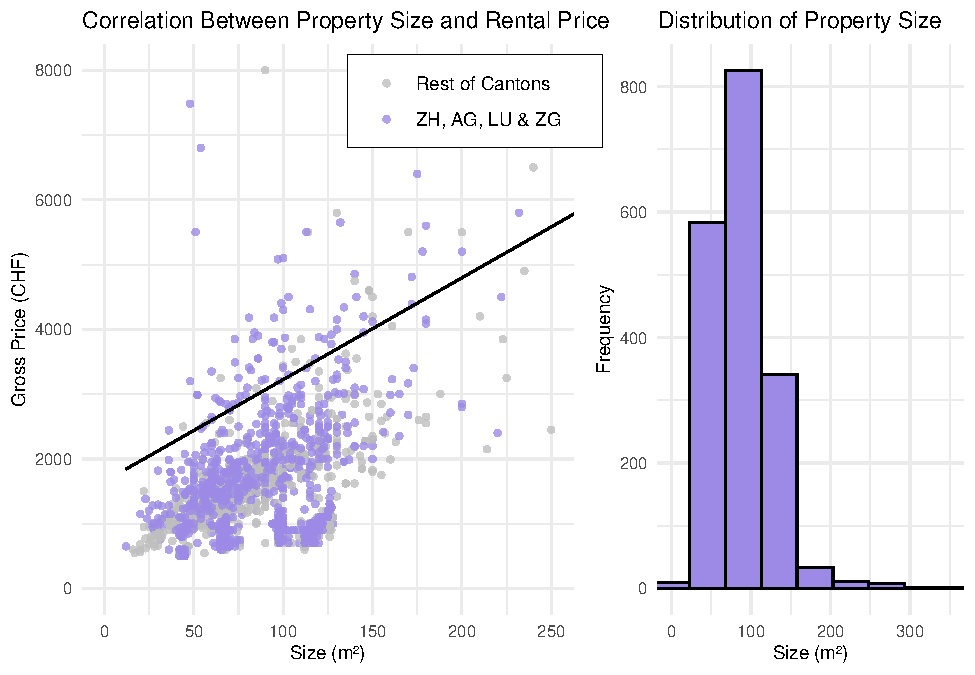
\includegraphics{2024_groupXX_report_files/figure-latex/Property Size and Rental Price-1.pdf}

\subsubsection{Influence of Number of Rooms on Rental
Price}\label{influence-of-number-of-rooms-on-rental-price}

\begin{itemize}
\tightlist
\item
  \textbf{Effect of Number of Rooms on Rental Price}
\end{itemize}

This scatter plot explores how the number of rooms affects the gross
rental price. While there is a general trend of increasing rental prices
with more rooms, the variability in price also increases, as indicated
by the spread of data points.

\begin{itemize}
\tightlist
\item
  \textbf{Distribution of Number of Rooms}
\end{itemize}

The bar chart illustrates the frequency of properties based on the
number of rooms. Properties with 3 to 4 rooms are the most common, which
aligns with the predominance of smaller property sizes seen in the
previous chart.

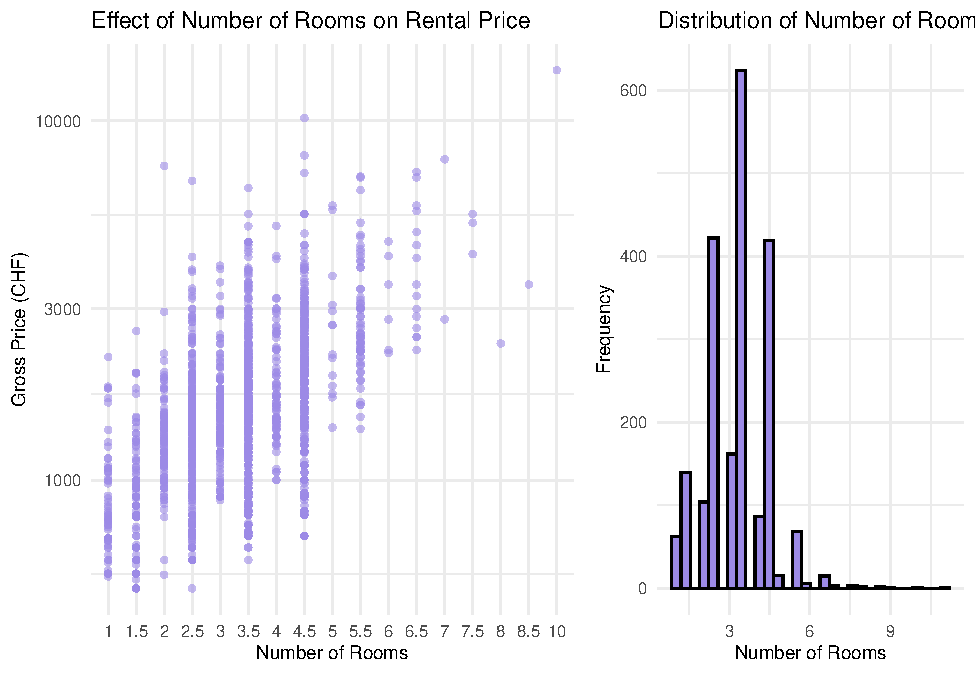
\includegraphics{2024_groupXX_report_files/figure-latex/Number of Rooms-1.pdf}

\section{Data Modeling}\label{data-modeling}

\emph{Complete}

\section{Linear Model}\label{linear-model}

\subsection{Purpose and Target}\label{purpose-and-target}

We decided to employ a linear regression model in order to predict
prices for different rental properties, specifically apartments. We
created three different models, each taking into account different
features to help us gain better insight.

\subsubsection{Linear Model 1}\label{linear-model-1}

The first model (\emph{all\_lm\_model}) takes all available property
features into account to train and make predictions. From this we were
able to see that some of those we included were not relevant to the
target variable, as seen below:

\emph{Click to see the summary of the first linear model}

\begin{verbatim}
## 
## Call:
## lm(formula = Price_Gross ~ ., data = train_set)
## 
## Residuals:
##     Min      1Q  Median      3Q     Max 
## -2836.4  -509.0  -115.9   268.6  8519.2 
## 
## Coefficients: (6 not defined because of singularities)
##                        Estimate Std. Error t value Pr(>|t|)    
## (Intercept)            -79.9609   139.5073  -0.573 0.566701    
## Canton_num2            322.2563   143.9988   2.238 0.025516 *  
## Canton_num3            -88.3072   158.5068  -0.557 0.577610    
## Canton_num4            431.1805    93.7620   4.599 4.98e-06 ***
## Days_Difference          4.5627     1.0754   4.243 2.48e-05 ***
## Customer_Segment_num2  379.5067   104.9582   3.616 0.000319 ***
## Category_num2         1324.3846   201.4030   6.576 8.99e-11 ***
## Nr_rooms               288.6288    35.5431   8.121 1.87e-15 ***
## Package_Product_num2   128.1776   139.4190   0.919 0.358194    
## Package_Product_num3   -25.5366   142.2814  -0.179 0.857609    
## Package_Product_num4         NA         NA      NA       NA    
## GDP_2020_21                  NA         NA      NA       NA    
## GDP_per                      NA         NA      NA       NA    
## Population                   NA         NA      NA       NA    
## Area_km2                     NA         NA      NA       NA    
## Density                      NA         NA      NA       NA    
## Size_m2                  2.4705     0.6631   3.726 0.000209 ***
## ---
## Signif. codes:  0 '***' 0.001 '**' 0.01 '*' 0.05 '.' 0.1 ' ' 1
## 
## Residual standard error: 881 on 761 degrees of freedom
## Multiple R-squared:  0.3678, Adjusted R-squared:  0.3595 
## F-statistic: 44.27 on 10 and 761 DF,  p-value: < 2.2e-16
\end{verbatim}

\emph{As we can see in the model summary, some variables are converted
into factors and interpreted separately, we can also see `Nr\_rooms' is
relevant in general, but Package\_Product and Category, for example, are
not.}

With this information we were able to refine our selection of variables
for training the following models, one with only a few variables, and
one with only one.

\subsubsection{Linear Model 2}\label{linear-model-2}

The next model ( \emph{few\_lm\_model} ) we trained with fewer dependent
variables, only those of high importance. For this one, we took into
account only the ones that were calculated to be significant to the
model's performance.

\emph{Click to see the summary of the second linear model}

\begin{verbatim}
## 
## Call:
## lm(formula = Price_Gross ~ ., data = rel_train_set)
## 
## Residuals:
##     Min      1Q  Median      3Q     Max 
## -2840.5  -504.6  -124.3   257.5  8518.7 
## 
## Coefficients:
##                        Estimate Std. Error t value Pr(>|t|)    
## (Intercept)            -86.0523   139.3439  -0.618 0.537054    
## Canton_num2            322.6111   143.7943   2.244 0.025147 *  
## Canton_num3            -84.3385   158.3760  -0.533 0.594520    
## Canton_num4            434.7715    93.6368   4.643 4.04e-06 ***
## Days_Difference          4.5514     1.0721   4.245 2.45e-05 ***
## Customer_Segment_num2  413.9179    74.1661   5.581 3.32e-08 ***
## Category_num2         1316.9668   200.4911   6.569 9.39e-11 ***
## Nr_rooms               289.5100    35.5155   8.152 1.47e-15 ***
## Size_m2                  2.4762     0.6628   3.736 0.000201 ***
## ---
## Signif. codes:  0 '***' 0.001 '**' 0.01 '*' 0.05 '.' 0.1 ' ' 1
## 
## Residual standard error: 880.6 on 763 degrees of freedom
## Multiple R-squared:  0.3667, Adjusted R-squared:  0.3601 
## F-statistic: 55.23 on 8 and 763 DF,  p-value: < 2.2e-16
\end{verbatim}

\emph{Here we can see that the variables taken into account were Canton,
Days\_Difference, Category, Customer\_Segment, Nr\_rooms and Size\_m2.}

\subsubsection{Linear Model 3}\label{linear-model-3}

The last model generated took into account only \emph{two} variable as a
predictor: \emph{Nr\_rooms} and \emph{Category\_num2}. The number of
rooms seems to have one of, if not the biggest effect on rental price of
a property, which is why we went with this variable for analysis. The
second customer category also has a significant effect, so it was
included.

\emph{Click to see the summary of the third linear model}

\begin{verbatim}
##                Estimate Std. Error   t value     Pr(>|t|)
## (Intercept)    442.3222  113.14728  3.909261 1.007483e-04
## Nr_rooms       354.0830   32.54504 10.879783 9.663820e-26
## Category_num2 1565.0616  209.67941  7.464069 2.274718e-13
\end{verbatim}

\subsection{Interpretation}\label{interpretation}

All three models offer us some insight into the behavior of rental
prices for different properties. Interestingly, our research thus far
shows that the Canton of said property is not that influential in its
rental price, except for Canton 3.

\emph{(Canton 1: Argau, Canton 2: Luzern, Canton 3: Zürich, Canton 4:
Zug)}

For desired results, we will focus on the second model, which includes
all the variables considered significant for the best results.

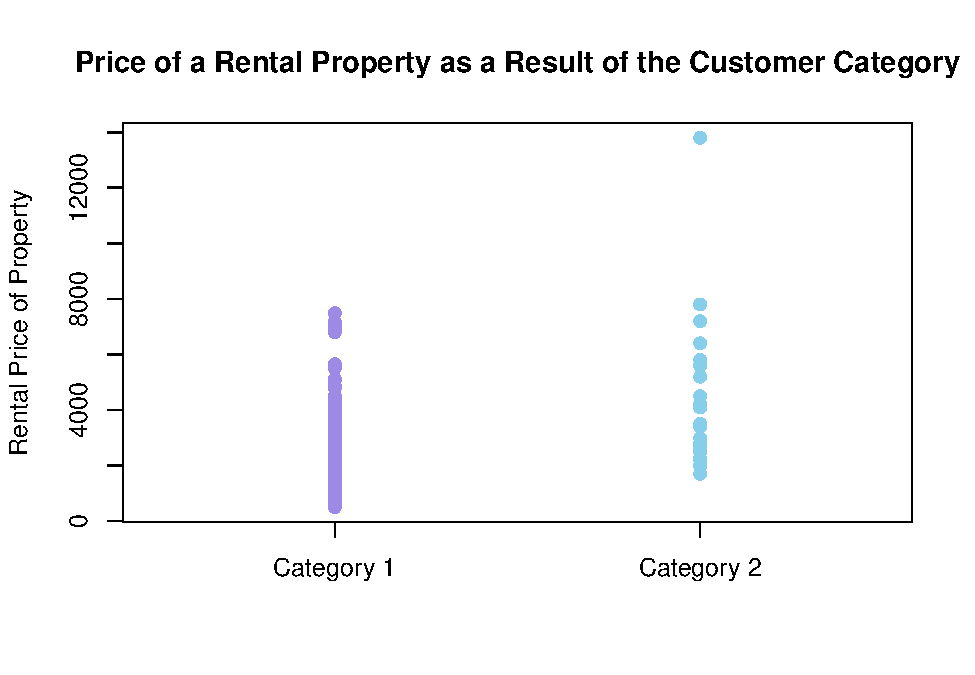
\includegraphics{2024_groupXX_report_files/figure-latex/LM Price Vs Category-1.pdf}

In this diagram we can observe that, though there are fewer instances of
Category 2 (House) compared to Category 1 (Apartment), Category 2
properties tend to have higher rental prices. This does not, however,
indicate that they may be the more lucrative option, as houses tend to
incur other costs that are either not present, or the cost is split in
the community, in the case of apartments.

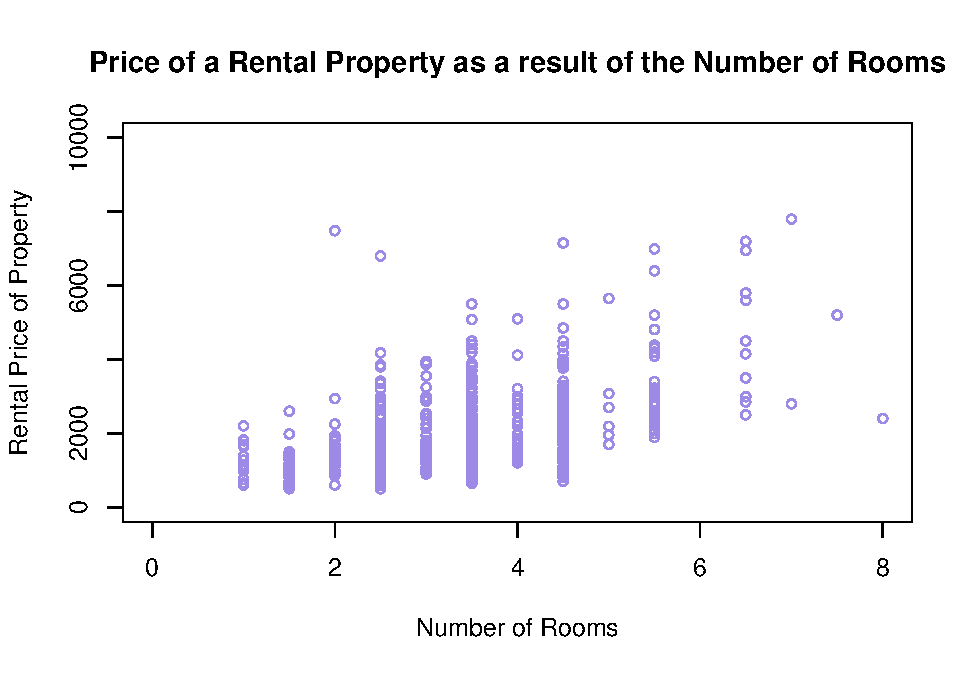
\includegraphics{2024_groupXX_report_files/figure-latex/LM First Model Plot-1.pdf}

In the illustration above, we depict the relationship between the number
of rooms in a property and the gross price of the same. We can observe
an upward trend, which leads to believe that a higher number of rooms
leads to a higher price, which would make sense. This information must
also be taken into consideration together with other variables, like the
property's area in meters squared, average size of rooms, location, etc.

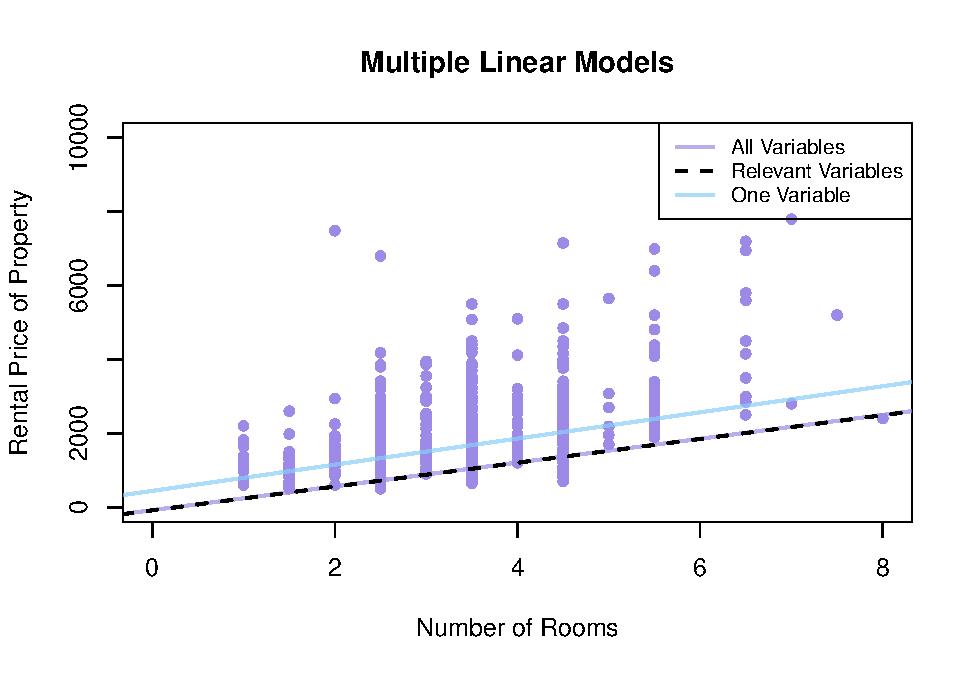
\includegraphics{2024_groupXX_report_files/figure-latex/3LM Plots-1.pdf}

\emph{Looking closely, we can see that the model with all variables, and
the one with relevant variables, have almost the exact same performance}

In the visual aid above, we can observe how each of these three models
compare to each other and the data. The model that takes into account
only the number of rooms as an independent variable is more generous
when predicting prices of properties. This does not mean, however, that
it is a better or worse model.

\subsection{Model Comparison}\label{model-comparison}

Next, we will take a look at how these models make predictions, and
compare them. Two of our models have been trained on practically the
same data, as seen in the previous visuals, where we outlined that the
first model is trained on ALL available variables in the data, and the
second model is trained only on the relevant variables. So far it seems
both of them will lead to very similar predictions, so we decided to
test that theory below.

\begin{table}[!h]
\centering\centering
\fontsize{10}{12}\selectfont
\begin{tabular}[t]{>{\raggedright\arraybackslash}p{3cm}|>{\raggedright\arraybackslash}p{2cm}|>{\raggedright\arraybackslash}p{2cm}|>{\raggedright\arraybackslash}p{2cm}|>{\raggedright\arraybackslash}p{2cm}|>{\raggedright\arraybackslash}p{2cm}|>{\raggedright\arraybackslash}p{2cm}}
\hline
\cellcolor[HTML]{9C8AE6}{\textcolor{white}{\textbf{Model}}} & \cellcolor[HTML]{9C8AE6}{\textcolor{white}{\textbf{RMSE}}} & \cellcolor[HTML]{9C8AE6}{\textcolor{white}{\textbf{MAE}}} & \cellcolor[HTML]{9C8AE6}{\textcolor{white}{\textbf{R\_Squared}}} & \cellcolor[HTML]{9C8AE6}{\textcolor{white}{\textbf{Adj\_R\_Squared}}} & \cellcolor[HTML]{9C8AE6}{\textcolor{white}{\textbf{AIC}}} & \cellcolor[HTML]{9C8AE6}{\textcolor{white}{\textbf{BIC}}}\\
\hline
\textbf{\cellcolor{gray!10}{All Variables}} & \cellcolor{gray!10}{952.4202} & \cellcolor{gray!10}{587.2066} & \cellcolor{gray!10}{0.3678088} & \cellcolor{gray!10}{0.3595014} & \cellcolor{gray!10}{12673.74} & \cellcolor{gray!10}{12729.53}\\
\hline
\textbf{Relevant Variables} & 951.5899 & 584.5305 & 0.3667123 & 0.3600723 & 12671.08 & 12717.57\\
\hline
\textbf{\cellcolor{gray!10}{One Variable}} & \cellcolor{gray!10}{1009.9926} & \cellcolor{gray!10}{673.3609} & \cellcolor{gray!10}{0.2746980} & \cellcolor{gray!10}{0.2728116} & \cellcolor{gray!10}{12763.81} & \cellcolor{gray!10}{12782.40}\\
\hline
\end{tabular}
\end{table}

As we can see from the models' two error metrics (\emph{MSE and RMSE}),
the models trained with more variables have a slightly better
performance on the test data. The R-Squared and Adjusted R-Squared
values indicate how well the model can explain variance in the data, and
the two initial models have performed better in this sense as well. As
far as AIC and BIC, we can see that though there is not much difference,
the model trained only on relevant variables slightly outperforms the
other two, indicating a better trade-off between model fit and
simplicity.

\subsection{Conclusion}\label{conclusion}

Our linear models suggest that properties, specifically houses, with
more rooms go for a higher price. This doesn't necessarily indicate that
they may be the best choice for renting out to customers, but it does
suggest that they are the properties which generate the highest gross
payment on a regular basis.

It is also made clear in our findings, that although the number of rooms
is a good indicator as to how much a property may be worth renting out
for, it is not necessarily the best way to go about this. Previously, we
saw that the model trained only on the number of rooms in a property
predicted higher rental prices than the other two. We cannot yet accept
that conclusion, as the only confident insight we have been able to find
is that a linear model is not the best fit for a problem that has so
many significant variables, as shown previously in the two initial
linear model summaries.

\section{GLM - Generalised Linear -
Binomial}\label{glm---generalised-linear---binomial}

\subsection{Purpose and Target}\label{purpose-and-target-1}

Quick sales or rentals are crucial for Zug Estates in the commercial
real estate world. Fast transactions minimize vacancy periods, ensuring
steady cash flow and maximizing returns on investment. This efficiency
not only benefits property owners by reducing holding costs but also
attracts potential clients who value quick and smooth processes.

We decided to use a Generalized Linear Model, Binomial to modelize it.

\subsection{Interpretation}\label{interpretation-1}

Before jumping into the model, we needed to do some adjustments to the
data:

\emph{Click to see the results}

\begin{verbatim}
## [1] 16.04944
\end{verbatim}

The average time it takes an owner to rent out a flat or house is 16
days. Therefore, we have taken the average as a reference, if a property
takes less than 17 days it is categorised as `Fast sale' and coded as 1,
otherwise it is coded as 0.

Then we decided to divide the data set (enc\_data) into two subsets: one
for training (train\_set) and another for testing (test\_set). The
training set is used to tune the model, while the test set is used to
evaluate the performance of the model. We will use it later.

In summary, the logistic regression model indicates that Price\_Gross,
certain Canton categories, and Customer\_Segment have significant
effects on the likelihood of a quick sale. Specifically, higher prices
decrease the probability, while certain regions (Canton\_num3 and
Canton\_num4) and customer segments have varying influences. The fit of
the model is reasonable, as indicated by the reduction in deviance and
the AIC value. Mas concreatmente, podemos extraer informacion muy
interesante que relfexionaremos tras analizar mas en profunidad el
modelo.

\begin{itemize}
\item
  \textbf{Price\_Gross:} The negative coefficient indicates that higher
  gross prices are associated with lower probabilities of a quick sale.
  This suggests that properties priced higher may take longer to sell,
  likely due to a smaller pool of potential buyers or perceived
  overvaluation. However the coefieicnete is so small que no se puede
  desestimar. Sorpresivamente para Zug Estates el precio no parece jugar
  un papel significativo.
\item
  \textbf{Nr\_rooms:} Not significant (p-value = 0.296563), which
  implies that the number of rooms may not be a decisive factor for
  quick sales in Central Switzerland.
\item
  \textbf{Size\_m2:} Not significant (p-value = 0.703451), thus, the
  size of the property alone does not strongly influence quick sales.
\item
  \textbf{Canton\_num:}

  \begin{itemize}
  \item
    \textbf{Canton\_num2:} Negative effect, not significant (p-value =
    0.07185)
  \item
    \textbf{Canton\_num3:} Positive effect, significant (p-value =
    0.006502)
  \item
    \textbf{Canton\_num4:} Positive effect, significant (p-value =
    0.000767)
  \end{itemize}
\end{itemize}

Properties in Canton\_num3 and Canton\_num4 have significantly higher
odds of quick sales, suggesting these areas are in high demand or have
market conditions conducive to faster transactions. This two canton are
equivalent to X and Y which mean that the probabilities of a quick sale
in Canton\_num3 are approximately 17.46 times greater than in the
reference canton and for Canton\_num4 are approximately 2.27 times
higher than in the baseline canton.

\emph{Click to see the results}

\begin{verbatim}
##           (Intercept)           Price_Gross              Nr_rooms 
##             3.9771674             0.9994328             1.1155637 
##               Size_m2           Canton_num2           Canton_num3 
##             1.0007269             0.5348910            17.4591650 
##           Canton_num4 Customer_Segment_num2         Category_num2 
##             2.2731286             0.3451728             2.3769725
\end{verbatim}

This is important for the Zug-based company's future property
operations.

Later we have added to the original dataset a new column named
fitted\_values to the training set (train\_set). This column contains
the predicted probabilities obtained from the fitted model. The fitted
values are the predicted probabilities that the dependent variable
(fast.sale) equals 1 (i.e., a quick sale) for each observation in the
training set.

\emph{Click to see the results}

\begin{verbatim}
## # A tibble: 6 x 2
##   fast.sale fitted_values
##       <dbl>         <dbl>
## 1         1         0.615
## 2         1         0.882
## 3         1         0.620
## 4         0         0.962
## 5         1         0.892
## 6         1         0.849
\end{verbatim}

Finally, we have made Predictions on the Test Set. The interpretation is
the interpretation of the actual outcome , if it was a quick sale (1) or
not (0). For example, in the first case, the model predicted a 78.5\%
probability of a quick sale. This prediction is quite accurate and
confident.

\emph{Click to see the results}

\begin{verbatim}
## # A tibble: 6 x 2
##   fast.sale fitted_values
##       <dbl>         <dbl>
## 1         1         0.785
## 2         0         0.431
## 3         1         0.792
## 4         1         0.790
## 5         1         0.676
## 6         1         0.785
\end{verbatim}

To measure the quality of the model so that Zug Estates can make
adequate predictions:

\emph{Click to see the results}

\begin{verbatim}
##          Actual
## Predicted     0     1
##         0  5.70  7.77
##         1 19.69 66.84
\end{verbatim}

\begin{verbatim}
##          Actual
## Predicted   0   1
##         0  11  15
##         1  38 129
\end{verbatim}

\subsection{Conclusion}\label{conclusion-1}

Without being exhaustive, here are some conclusions about the model:

\begin{itemize}
\item
  \textbf{False Negatives (FN):} The model incorrectly predicted 15
  instances as not quick sales (0) when they were quick sales (1), which
  is 7.77\% of the total predictions. This indicates missed
  opportunities where the model failed to identify actual quick sales.
\item
  \textbf{True Positives (TP):} The model correctly predicted 129
  instances as quick sales (1), which is 66.84\% of the total
  predictions. This shows a strong performance in correctly identifying
  quick sales.
\end{itemize}

Finally, with respect to performance metrics that are standard in
Machine Learning:

\emph{Click to see the results}

\begin{verbatim}
## [1] "Precision: 0.772455089820359"
\end{verbatim}

\begin{verbatim}
## [1] "Recall: 0.895833333333333"
\end{verbatim}

\begin{verbatim}
## [1] "Accuracy: 0.725388601036269"
\end{verbatim}

\begin{itemize}
\item
  \textbf{Precision} indicates how reliable the model is when it
  predicts a quick sale. With a precision of 77.2\%, the model has a
  moderate false positive rate, meaning some of the predicted quick
  sales are actually not quick sales.
\item
  \textbf{Recall} measures how well the model identifies actual quick
  sales. With a high recall of 89.6\%, the model successfully identifies
  most of the quick sales, indicating a low false negative rate.
\item
  \textbf{Accuracy} provides an overall assessment of model performance.
  With an accuracy of 72.5\%, the model correctly predicts the outcome
  for a majority of the cases but still makes errors in a significant
  number of cases.
\end{itemize}

\section{GLM - Generalised Linear -
Poisson}\label{glm---generalised-linear---poisson}

\subsection{Purpose and Target}\label{purpose-and-target-2}

Following the line of what was written on these lines, we want to
provide Zug estates with a tool that allows predicting how many rooms
would need a house to fit a market. For this we will use Quasi Poisson
model, which is a variant of the Poisson regression model that is used
to handle overdispersion in the data. Instead of assuming that the
variance is equal to the mean (as in Poisson), the quasi-Poisson model
allows the variance to be a function of the mean, but more flexible.

For Zug Estates, understanding what properties are in demand is key. By
predicting the number of rooms accurately, they can sell or rent
properties faster. This reduces vacancy periods, keeps cash flow steady,
and boosts investment returns. It also lowers holding costs and speeds
up transactions, making property owners and clients happy with quick,
smooth processes.

\subsection{Interpretation}\label{interpretation-2}

We decided to perform a logarithmic transformation on specific columns
within two data sets: train\_set and test\_set. By applying these
transformations, our code is preparing the train\_set and test\_set for
better performance in subsequent glm model.

\emph{Click to see the code}

Here the \textbf{model}:

\emph{Click to see the code}

The model takes into account a previous logarithmic transformation that
we have done so it must be interpreted in those terms, since it must fit
what we want to put into it. The relevance of the price and the square
meters in addition to one of the cantons to calculate the number of
rooms is attested by the p value having statistical significance.
However, whether or not the apartment is being rented by a professional
or several of the cantons is not relevant, since its value is greater
than 0.05.

When interpreting the price, for example, we can see that a 1\% increase
in Size\_m2 increases the expected count of rooms by
𝑒0.00593205≈1.00593, or approximately 0.593\%.

\begin{itemize}
\item
  Each point on the scatter plot represents a pair of actual and
  predicted values for a particular observation in the test set.
\item
  The red line is the line of perfect prediction, where the predicted
  values would exactly equal the actual values (i.e.,
  {[}Ecuación{]}y=x). Ideally, all points would lie on this line if the
  model predictions were perfect.
\end{itemize}

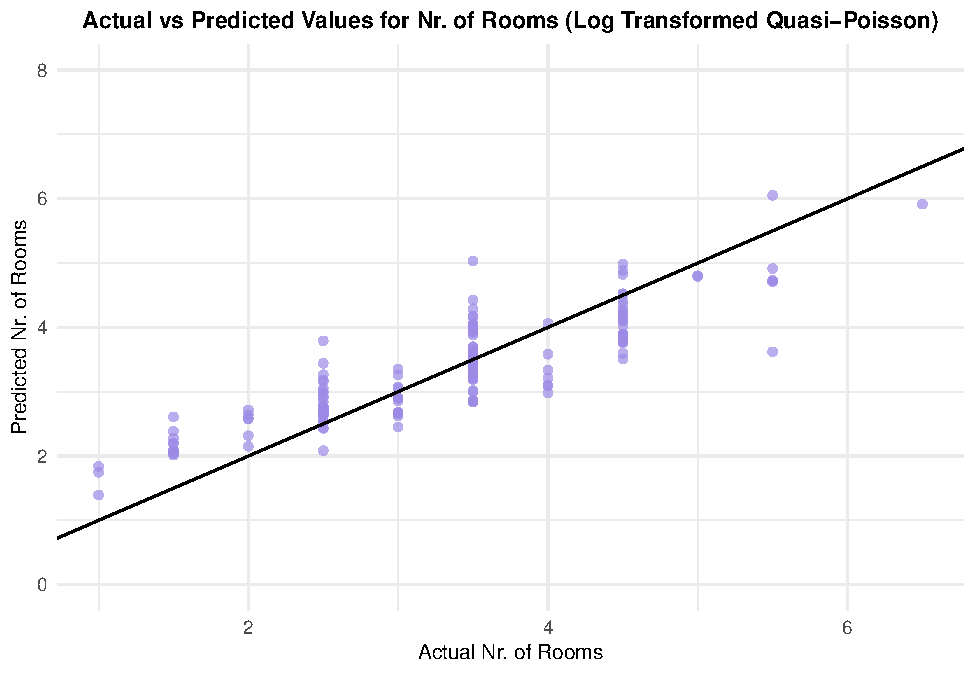
\includegraphics{2024_groupXX_report_files/figure-latex/GLM Poisson 3-1.pdf}

This scatter plot demonstrates that the Quasi-Poisson model with
log-transformed predictors effectively captures the overall trend. As
the actual number of rooms increases, the predicted values also rise
correspondingly, indicating that the model successfully identifies the
general relationship between the predictors and the target variable.

The trend highlights the model's capability to generalize well across
the range of data points, reflecting a solid understanding of the
underlying patterns in the dataset.

Despite some deviations from the line of perfect prediction (in red,),
the model shows a promising performance. The increasing dispersion of
points with higher actual values suggests that while the model is less
precise for larger counts of rooms, it still maintains a coherent
predictive behavior.

\section{GAM - Generalised Additive
Model}\label{gam---generalised-additive-model}

\subsection{Purpose and Target}\label{purpose-and-target-3}

\subsubsection{Purpose}\label{purpose}

The purpose is to analyze and model the relationship between property
size (in square meters) and price using various statistical techniques.
The goal is to determine the best-fitting model that accurately predicts
property prices based on the available data. By fitting and comparing
different models Generalized Additive Models (GAMs), we aim to identify
the most reliable and insightful model. Additionally, the report
provides recommendations for further improving the model and making more
accurate predictions.

\begin{itemize}
\item
  \textbf{Data Analysis:} Understand the dataset and the key variables
  involved.
\item
  \textbf{Model Fitting:} Apply different statistical models to the
  data.
\item
  \textbf{Model Comparison:} Evaluate and compare the performance of the
  models.
\item
  \textbf{Recommendations:} Provide suggestions for future improvements
  and next steps.
\end{itemize}

\subsection{Interpretation}\label{interpretation-3}

\subsubsection{Quadratic Model Plot}\label{quadratic-model-plot}

The graph shows the relationship between Size\_m2 and Price\_Gross using
a quadratic model. The black line represents the fitted values from the
quadratic model, and the shaded area represents the confidence interval
around the fitted values.

\textbf{Key Observations}

\begin{itemize}
\item
  \textbf{Non-linear Relationship} between Size\_m2 and Price\_Gross.
  Initially, Price\_Gross increases with Size\_m2 up to about 300-400
  m², after which it starts to decrease.
\item
  \textbf{The Confidence Intervals} widen significantly beyond 300 m²,
  indicating increased uncertainty in the predictions for larger
  properties. This suggests that the model is less reliable for larger
  properties due to fewer data points in this range.
\item
  \textbf{Data Distribution.} Most of the data points are clustered
  below 300 m², with few data points for larger properties. The fit of
  the model is more certain where there are more data points, and less
  certain where data points are sparse.
\end{itemize}

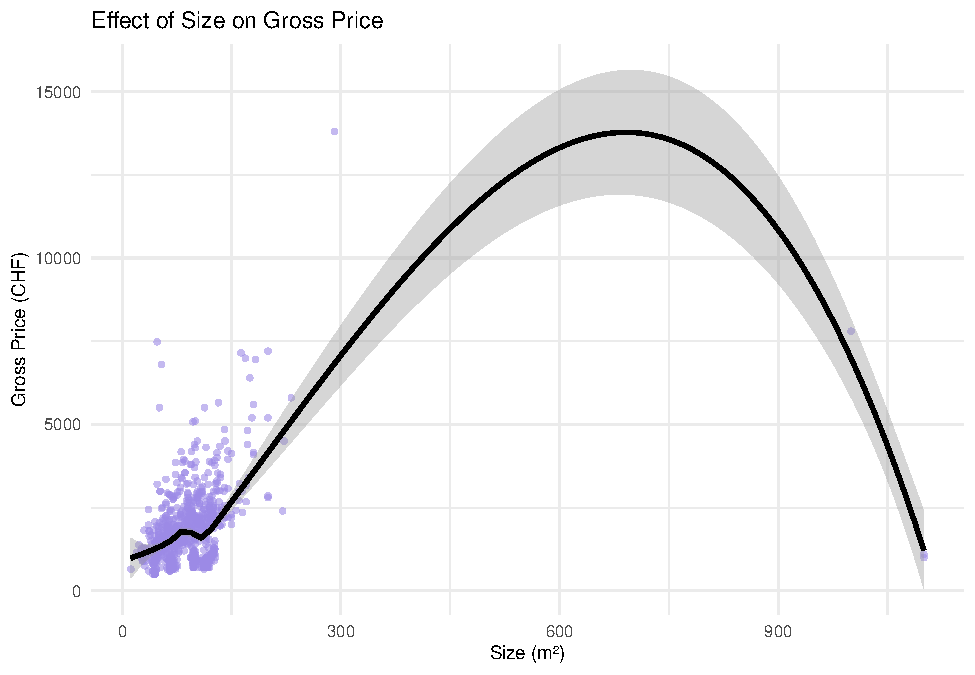
\includegraphics{2024_groupXX_report_files/figure-latex/GAM code 1 -1.pdf}

\textbf{Next Steps for the GAM}

Given the observations from the quadratic model, we can take the
following steps to improve our model using GAM:

\begin{itemize}
\item
  \textbf{Filter the data.} Consider filtering the data to include only
  properties with Size\_m2 less than 300 m². This can help improve the
  reliability of the model in the range where we have more data.
\item
  \textbf{Transform variables.} Transform Size\_m2 to log(Size\_m2) if a
  log transformation better captures the relationship and stabilises the
  variance.
\item
  \textbf{Include interactions} with other significant variables such as
  Nr\_rooms to capture more complex relationships.
\item
  \textbf{Use smoothing splines in GAM}, which can capture non-linear
  relationships more flexibly than a quadratic model.
\end{itemize}

Once these parameters are clear, we will implement them in our GAM
models and see which ones perform best.

\subsubsection{Basic GAM}\label{basic-gam}

Starting with fitting a basic GAM to capture more complex non-linear
relationships:

Click to see the summary

\begin{verbatim}
## 
## Family: gaussian 
## Link function: identity 
## 
## Formula:
## Price_Gross ~ s(Size_m2)
## 
## Parametric coefficients:
##             Estimate Std. Error t value Pr(>|t|)    
## (Intercept)  1700.68      27.82   61.13   <2e-16 ***
## ---
## Signif. codes:  0 '***' 0.001 '**' 0.01 '*' 0.05 '.' 0.1 ' ' 1
## 
## Approximate significance of smooth terms:
##              edf Ref.df     F p-value    
## s(Size_m2) 8.907  8.997 68.76  <2e-16 ***
## ---
## Signif. codes:  0 '***' 0.001 '**' 0.01 '*' 0.05 '.' 0.1 ' ' 1
## 
## R-sq.(adj) =  0.389   Deviance explained = 39.5%
## GCV = 7.5459e+05  Scale est. = 7.4684e+05  n = 965
\end{verbatim}

\emph{R-squared (adj.): 0.389, indicating that 38.9\% of the variability
is explained. Deviance explained: 39.5\%.}

\subsubsection{GAM with Multiple
Predictors}\label{gam-with-multiple-predictors}

To account for additional factors, a GAM including multiple predictors
was fitted:

Click to see the summary

\begin{verbatim}
## 
## Family: gaussian 
## Link function: identity 
## 
## Formula:
## Price_Gross ~ s(Size_m2) + Days_Difference + Nr_rooms + GDP_per + 
##     Population + Area_km2 + Density
## 
## Parametric coefficients:
##                   Estimate Std. Error t value Pr(>|t|)    
## (Intercept)     -2.429e-03  1.726e-03  -1.407   0.1597    
## Days_Difference  6.473e+00  8.729e-01   7.415 2.68e-13 ***
## Nr_rooms         2.704e+02  5.213e+01   5.188 2.60e-07 ***
## GDP_per          5.979e-03  3.404e-03   1.757   0.0793 .  
## Population       9.380e-04  4.846e-04   1.936   0.0532 .  
## Area_km2         1.054e-01  1.457e-01   0.723   0.4698    
## Density         -1.579e+00  1.068e+00  -1.479   0.1395    
## ---
## Signif. codes:  0 '***' 0.001 '**' 0.01 '*' 0.05 '.' 0.1 ' ' 1
## 
## Approximate significance of smooth terms:
##              edf Ref.df    F p-value    
## s(Size_m2) 5.146  5.981 32.5  <2e-16 ***
## ---
## Signif. codes:  0 '***' 0.001 '**' 0.01 '*' 0.05 '.' 0.1 ' ' 1
## 
## Rank: 13/16
## R-sq.(adj) =  0.413   Deviance explained = 41.9%
## GCV = 7.2697e+05  Scale est. = 7.1857e+05  n = 965
\end{verbatim}

\emph{Adjusted R-squared: 0.413, indicating 41.3\% of variability is
explained. Significant predictors: Days\_Difference, Nr\_rooms,
GDP\_per, Population.}

\subsubsection{Filtered GAM}\label{filtered-gam}

To focus on properties with Size\_m2 less than 300, a filtered GAM was
fitted:

Click to see the summary

\begin{verbatim}
## 
## Family: gaussian 
## Link function: identity 
## 
## Formula:
## Price_Gross ~ s(Size_m2) + Days_Difference + Nr_rooms + GDP_per + 
##     Population + Area_km2 + Density
## 
## Parametric coefficients:
##                   Estimate Std. Error t value Pr(>|t|)    
## (Intercept)     -2.343e-03  1.684e-03  -1.392   0.1643    
## Days_Difference  6.003e+00  8.577e-01   6.999 4.88e-12 ***
## Nr_rooms         2.495e+02  5.169e+01   4.827 1.62e-06 ***
## GDP_per          6.803e-03  3.316e-03   2.051   0.0405 *  
## Population       8.362e-04  4.731e-04   1.767   0.0775 .  
## Area_km2         1.708e-01  1.433e-01   1.192   0.2336    
## Density         -1.550e+00  1.041e+00  -1.489   0.1367    
## ---
## Signif. codes:  0 '***' 0.001 '**' 0.01 '*' 0.05 '.' 0.1 ' ' 1
## 
## Approximate significance of smooth terms:
##              edf Ref.df    F p-value    
## s(Size_m2) 7.514  7.916 35.2  <2e-16 ***
## ---
## Signif. codes:  0 '***' 0.001 '**' 0.01 '*' 0.05 '.' 0.1 ' ' 1
## 
## Rank: 14/16
## R-sq.(adj) =  0.431   Deviance explained = 43.9%
## GCV = 6.8502e+05  Scale est. = 6.754e+05  n = 962
\end{verbatim}

\emph{Adjusted R-squared: 0.431, explaining 43.1\% of variability.}

\subsubsection{Log-Transformed GAM}\label{log-transformed-gam}

A log transformation of Size\_m2 was applied to improve model fit:

Click to see the summary

\begin{verbatim}
## 
## Family: gaussian 
## Link function: identity 
## 
## Formula:
## Price_Gross ~ s(log_Size_m2) + Days_Difference + Nr_rooms + GDP_per + 
##     Population + Area_km2 + Density
## 
## Parametric coefficients:
##                   Estimate Std. Error t value Pr(>|t|)    
## (Intercept)     -3.466e-03  1.763e-03  -1.966   0.0496 *  
## Days_Difference  5.769e+00  8.992e-01   6.415 2.22e-10 ***
## Nr_rooms         3.492e+02  5.224e+01   6.684 3.96e-11 ***
## GDP_per          6.650e-03  3.482e-03   1.910   0.0565 .  
## Population       1.260e-03  4.943e-04   2.548   0.0110 *  
## Area_km2        -6.384e-02  1.472e-01  -0.434   0.6646    
## Density         -2.169e+00  1.091e+00  -1.988   0.0471 *  
## ---
## Signif. codes:  0 '***' 0.001 '**' 0.01 '*' 0.05 '.' 0.1 ' ' 1
## 
## Approximate significance of smooth terms:
##                  edf Ref.df     F p-value    
## s(log_Size_m2) 7.438  7.877 23.15  <2e-16 ***
## ---
## Signif. codes:  0 '***' 0.001 '**' 0.01 '*' 0.05 '.' 0.1 ' ' 1
## 
## Rank: 14/16
## R-sq.(adj) =  0.388   Deviance explained = 39.6%
## GCV = 7.5932e+05  Scale est. = 7.4874e+05  n = 965
\end{verbatim}

\emph{Adjusted R-squared: 0.388, explaining 38.8\% of variability.}

\subsubsection{GAM with Interactions}\label{gam-with-interactions}

To explore interactions, a GAM including interaction terms was fitted:

Click to see the summary

\begin{verbatim}
## 
## Family: gaussian 
## Link function: identity 
## 
## Formula:
## Price_Gross ~ s(Size_m2) + Days_Difference + Nr_rooms + GDP_per + 
##     Population + Area_km2 + Density + s(Size_m2, by = Nr_rooms)
## 
## Parametric coefficients:
##                   Estimate Std. Error t value Pr(>|t|)    
## (Intercept)     -1.592e-03  1.683e-03  -0.946   0.3445    
## Days_Difference  6.204e+00  8.492e-01   7.305 5.87e-13 ***
## Nr_rooms         2.072e+02  1.668e+02   1.242   0.2144    
## GDP_per          5.362e-03  3.310e-03   1.620   0.1056    
## Population       6.345e-04  4.724e-04   1.343   0.1795    
## Area_km2         2.345e-01  1.419e-01   1.652   0.0989 .  
## Density         -1.099e+00  1.041e+00  -1.056   0.2912    
## ---
## Signif. codes:  0 '***' 0.001 '**' 0.01 '*' 0.05 '.' 0.1 ' ' 1
## 
## Approximate significance of smooth terms:
##                       edf Ref.df     F  p-value    
## s(Size_m2)          2.226  2.360 11.13 0.000302 ***
## s(Size_m2):Nr_rooms 7.018  7.463 38.82  < 2e-16 ***
## ---
## Signif. codes:  0 '***' 0.001 '**' 0.01 '*' 0.05 '.' 0.1 ' ' 1
## 
## Rank: 16/26
## R-sq.(adj) =  0.449   Deviance explained = 45.7%
## GCV = 6.8369e+05  Scale est. = 6.7338e+05  n = 965
\end{verbatim}

\emph{Adjusted R-squared: 0.449, explaining 44.9\% of variability.
Significant interaction: s(Size\_m2):Nr\_rooms.}

\subsection{Conclusion}\label{conclusion-2}

\subsubsection{Model Comparison Table}\label{model-comparison-table}

As can be seen in the table and in the summaries of each model, based on
the adjusted R-squared and the explained variance, the best fitting
model is the GAM with interaction terms.

This model explains 44.9\% of the variability in Price\_Gross and
includes significant interactions between \textbf{Size\_m2} and
\textbf{Nr\_rooms}.

\begin{table}[!h]
\centering\centering
\fontsize{10}{12}\selectfont
\begin{tabular}[t]{>{\raggedright\arraybackslash}p{3cm}|>{\raggedright\arraybackslash}p{2cm}|>{\raggedright\arraybackslash}p{2cm}|>{\raggedright\arraybackslash}p{2cm}}
\hline
\cellcolor[HTML]{9C8AE6}{\textcolor{white}{\textbf{Model}}} & \cellcolor[HTML]{9C8AE6}{\textcolor{white}{\textbf{R\_squared\_Adj}}} & \cellcolor[HTML]{9C8AE6}{\textcolor{white}{\textbf{Deviance\_Explained}}} & \cellcolor[HTML]{9C8AE6}{\textcolor{white}{\textbf{GCV\_Score}}}\\
\hline
\textbf{\cellcolor{gray!10}{GAM - Size\_m2}} & \cellcolor{gray!10}{0.389} & \cellcolor{gray!10}{39.5\%} & \cellcolor{gray!10}{754590}\\
\hline
\textbf{GAM - Full} & 0.413 & 41.9\% & 726970\\
\hline
\textbf{\cellcolor{gray!10}{GAM - Filtered}} & \cellcolor{gray!10}{0.431} & \cellcolor{gray!10}{43.9\%} & \cellcolor{gray!10}{685020}\\
\hline
\textbf{GAM - Log} & 0.388 & 39.6\% & 759320\\
\hline
\textbf{\cellcolor{gray!10}{GAM - Interaction}} & \cellcolor{gray!10}{0.449} & \cellcolor{gray!10}{45.7\%} & \cellcolor{gray!10}{683690}\\
\hline
\end{tabular}
\end{table}

\subsubsection{Next Steps}\label{next-steps}

\textbf{1. Higher-Order Polynomial Terms:} Explore cubic or higher-order
terms.

\textbf{2. Advanced GAMs:} Consider fitting more complex GAMs with
different smoothing parameters.

\textbf{3. Additional Predictors:} Include more relevant predictors to
improve model accuracy.

\textbf{4. Cross-Validation:} Perform cross-validation to validate model
robustness.

These steps will help in further refining the model and ensuring more
accurate predictions for property prices.

\subsection{Model Predictions}\label{model-predictions}

The analysis aims to forecast rental prices for houses and apartments.
Noticing that the highest volume of rental prices falls within the range
of 50 to 150 square meters, we have decided to focus our prediction on
rental prices within this segment. This size range can be understood as
a key market segment for Zug Estates, given its commercial relevance.

\textbf{Methodology used}

\begin{itemize}
\item
  \textbf{Cross-validation:} A 10-fold cross-validation was used to
  increase the robustness of the model, involving repeated training and
  testing.
\item
  \textbf{Model fitting:} as we have seen in the Model Comparison Table,
  we choosed the GAM - Interaction Model which included between its
  predictors including property size, listing period, number of rooms,
  GDP per capita, population, area and population density, and an
  interaction between property size and number of rooms.
\end{itemize}

\textbf{Performance metrics}

\begin{itemize}
\tightlist
\item
  \textbf{RMSE:} The accuracy of the model in predicting rental prices
  was measured by the RMSE, which averaged CHF 1005.04 across all
  replicates, indicating the model's predictive ability.
\end{itemize}

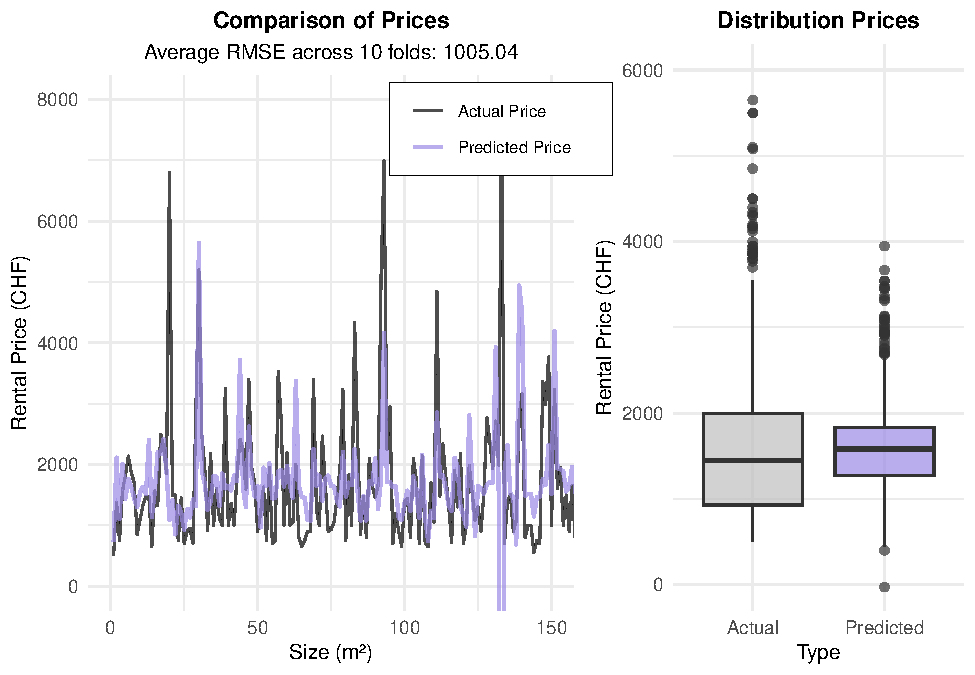
\includegraphics{2024_groupXX_report_files/figure-latex/GAM Plot-1.pdf}

\textbf{Results}

\begin{itemize}
\item
  \textbf{Price comparison:} Visual comparison showed the variability
  between predicted (purple) and actual (black) prices, with some
  variation across different property sizes.
\item
  \textbf{Price distribution:} Predicted prices showed a narrower
  interquartile range and fewer extremes compared to actual prices,
  suggesting under-prediction of outliers.
\end{itemize}

To conclude we can say that The GAM model is reasonably effective at
predicting rental prices for smaller properties, capturing general
trends despite some variation.

\textbf{Recommendations}

\begin{itemize}
\item
  \textbf{Refine the model:} Consider additional predictors or
  interactions to improve accuracy.
\item
  \textbf{Outlier analysis:} Investigate causes of outliers to refine
  predictions.
\item
  \textbf{Focus on target segment:} Ensure data accuracy for properties
  under 150 square metres to align with market interest.
\end{itemize}

This foundational analysis helps Zug Estates refine rental price
predictions to maintain competitiveness and market insight.

\section{Neural Network}\label{neural-network}

\subsection{Purpose and Target}\label{purpose-and-target-4}

When considering using a Neural Network, we decided to identify
potential high value properties within the dataset. To do this, we
engineered a new, binary column, identifying whether a property was
considered ``High-Ticket'' or not. In order to categorize properties
this way, we calculated the price per meter squared of each property,
and those in the top quartile had their High\_Ticket column value set to
1, others to 0.

With this transformation, we had created a binary classification
problem: is this property a high-ticket property? Answering this
question will allow us to filter out most properties which may not be as
lucrative for Zug Estates, and offer only the cream of the crop as
possible targets for acquisition.

\subsection{Interpretation}\label{interpretation-4}

After classifying the properties into either category, we were able to
analyze the model's performance on the dataset. If successful, this
Neural Network will be a great tool in the future to predict a possible
acquisition's performance over time. Properties may be acquired at lower
prices, and may not be very attractive at the time of purchase, but with
some remodeling and updating the living space, its perceived value may
be brought to a new high. This is what we try to predict with this
model: the potential of a specific property and to discern if it could
be a lucrative investment for Zug Estates.

\begin{table}[!h]
\centering\centering
\fontsize{10}{12}\selectfont
\begin{tabular}[t]{l|>{\centering\arraybackslash}p{4cm}|c}
\hline
\cellcolor[HTML]{9C8AE6}{\textcolor{white}{\textbf{ }}} & \cellcolor[HTML]{9C8AE6}{\textcolor{white}{\textbf{Actual: Non-High Ticket}}} & \cellcolor[HTML]{9C8AE6}{\textcolor{white}{\textbf{Actual: High-Ticket}}}\\
\hline
\cellcolor{gray!10}{Predicted: Non-High Ticket} & \cellcolor{gray!10}{142} & \cellcolor{gray!10}{7}\\
\hline
Predicted: High Ticket & 0 & 44\\
\hline
\end{tabular}
\end{table}

\emph{Confusion Matrix of the Neural Network's performance.}

As seen in the previous matrix, the model's performance on categorizing
properties into possible high-ticket or not is quite good, with only a
total of 7 (3.6\%) incorrect classifications. This tool will help in the
future, when looking at new properties, to have an idea of more or less
how lucrative a specific property could be to Zug Estates' portfolio.

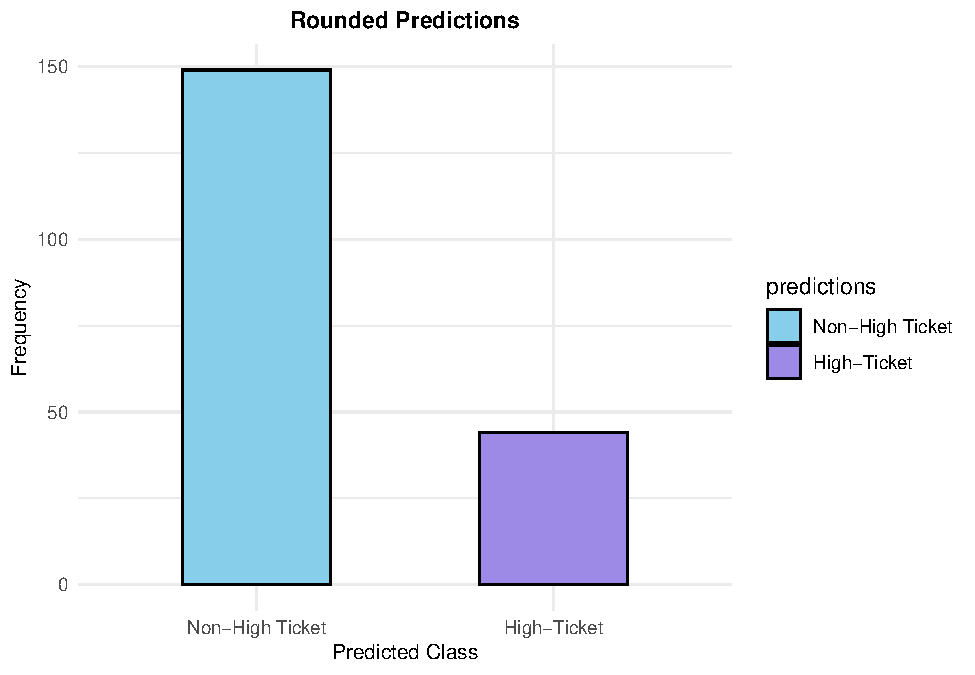
\includegraphics{2024_groupXX_report_files/figure-latex/NN Predictions Chart-1.pdf}

\emph{Predictions have been rounded because some values fell into
decimal places, due to the nature of the Neural Networks' activation
function (sigmoid curve)}

As we can see, not many values actually fall into the category of
High-Ticket properties, so having a tool like this network will be
beneficial in catching such opportunities early on and maximizing added
value and profits for the real estate company.

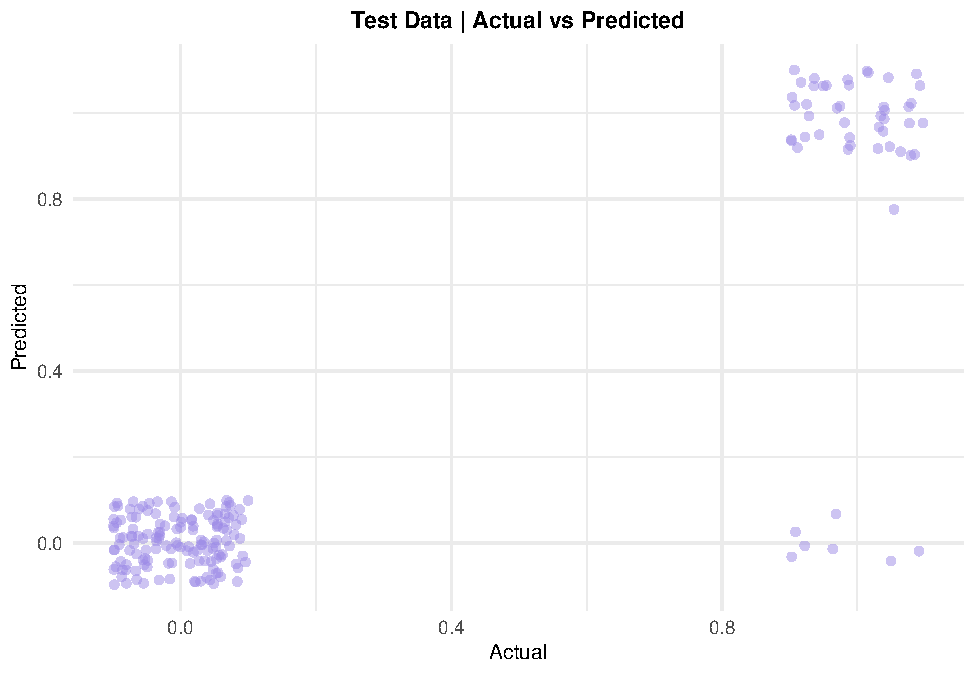
\includegraphics{2024_groupXX_report_files/figure-latex/NN Predictions Visual-1.pdf}

\emph{In this visual we can better appreciate the behavior of the
model's predictions. Jitter has been added to the values to avoid
overplotting (All values on a single coordinate)}

As we can see, the clusters near (0,0) and (1,1) show us correct
predictions made by the model. The small cluster on the bottom right
(near (1,0)) shows us the mistakes. This graph gives us a similar
representation to the confusion matrix, but also represents a visual
estimate to prediction errors. We can see from the clearly defined
clusters that our model is very confident in its predictions, and not
many incorrect predictions were made.

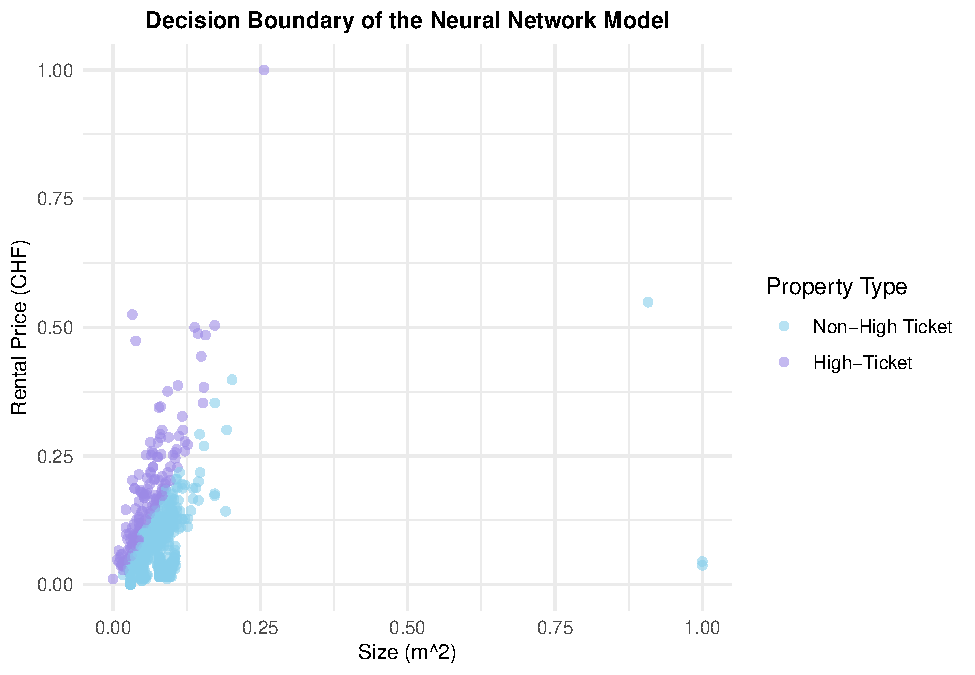
\includegraphics{2024_groupXX_report_files/figure-latex/NN Decision Boundary-1.pdf}
\emph{Values have been normalized between 0 and 1 to allow for better
visualization}

Here we can more clearly appreciate where the model has drawn its
decision boundary. With this information, we conclude that the neural
network model has clearly understood how to separate the properties
between High-Ticket and not. In the purple section, we see the models
classified as High-Ticket, which as is displayed, tend to be those with
a higher ``density'' of price per square meter. For Zug Estates, this
line represents the boundary between properties that may yield better
financial results (purple) and those that may not be so profitable
(blue). The fact that we can clearly distinguish them means that the
model can as well, and that it can recognize a clear difference between
possible high-ticket properties and those that may be more mediocre.

\subsection{Conclusion}\label{conclusion-3}

A Neural Network proves to be a very versatile tool when it comes to
adapting to data. This may be beneficial in the future, if this tool is
to be implemented and retrained/exposed to new properties in order to
provide some suggestions as to which to consider acquiring.

Having a tool such as this in Zug Estates' arsenal will most definitely
provide an edge over the competition, as identifying higher value
candidates for purchase will become faster and more efficient, helping
the team close profitable deals in a quicker fashion.

\section{Support Vector Machine}\label{support-vector-machine}

\subsection{Purpose and Target}\label{purpose-and-target-5}

Though the Neural Network presented great results, we wanted to make
sure to validate that it was the optimal choice for classification in
our case. Support Vector Machines (SVMs henceforth) also excel at binary
classification problems, so we wanted to create one and train it on the
same data in order to visualize and compare performance, to ensure we
use the better performing model for recommending properties to acquire.

In short, we want to make sure we offer Zug Estates the best option when
it comes to predicting performance of possible acquisitions. Our effort
comes to life by being thorough with our research, and comparing
different models to suggest the better one for the problem. In this
case, we compare the ability of a Neural Network and a SVM to recognize
potential high-value properties.

\subsection{Interpretation}\label{interpretation-5}

\textbf{Neural Network Performance}

\begin{table}[!h]
\centering\centering
\fontsize{10}{12}\selectfont
\begin{tabular}[t]{l|>{\centering\arraybackslash}p{4cm}|c}
\hline
\cellcolor[HTML]{9C8AE6}{\textcolor{white}{\textbf{ }}} & \cellcolor[HTML]{9C8AE6}{\textcolor{white}{\textbf{Actual: Non-High Ticket}}} & \cellcolor[HTML]{9C8AE6}{\textcolor{white}{\textbf{Actual: High-Ticket}}}\\
\hline
\cellcolor{gray!10}{Predicted: Non-High Ticket} & \cellcolor{gray!10}{142} & \cellcolor{gray!10}{7}\\
\hline
Predicted: High Ticket & 0 & 44\\
\hline
\end{tabular}
\end{table}

\textbf{SVM Performance}

\begin{table}[!h]
\centering\centering
\fontsize{10}{12}\selectfont
\begin{tabular}[t]{l|>{\centering\arraybackslash}p{4cm}|c}
\hline
\cellcolor[HTML]{9C8AE6}{\textcolor{white}{\textbf{ }}} & \cellcolor[HTML]{9C8AE6}{\textcolor{white}{\textbf{Actual: Non-High Ticket}}} & \cellcolor[HTML]{9C8AE6}{\textcolor{white}{\textbf{Actual: High-Ticket}}}\\
\hline
\cellcolor{gray!10}{Predicted: Non-High Ticket} & \cellcolor{gray!10}{143} & \cellcolor{gray!10}{8}\\
\hline
Predicted: High Ticket & 2 & 40\\
\hline
\end{tabular}
\end{table}

As we can see, comparing the two confusion matrices of both models, the
Neural Network has slightly better accuracy than the SVM. Though at
first glance it may seem like the better option, there are several
advantages and disadvantages between the models, which we will go over
shortly.

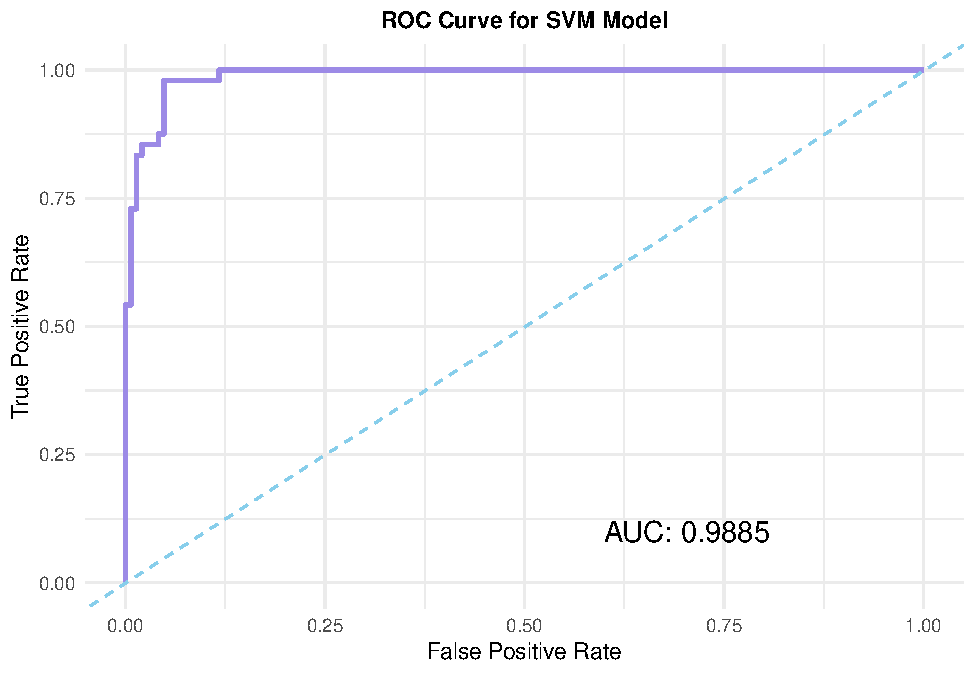
\includegraphics{2024_groupXX_report_files/figure-latex/SVM ROC Curve-1.pdf}

An SVM is particularly effective when working with higher-dimensional
data, and has better memory efficiency. It is also more robust to
over-fitting, but are less efficient with larger datasets because of the
training complexity. In our case however, we interpret the ROC Curve's
shape as well as the are-under-curve (AUC = 0.9885) to be excellent. The
SVM is adapting very well to the data, and has very strong
discriminative power.

Neural networks on the other hand, are more flexible and powerful when
it comes to approximating trends. They can also learn and extract
features that are not present in the data, finding new relationships
that may not be obvious, but can be very computationally intensive.

\begin{table}[!h]
\centering\centering
\fontsize{10}{12}\selectfont
\begin{tabular}[t]{>{\centering\arraybackslash}p{3cm}|>{\centering\arraybackslash}p{2cm}}
\hline
\cellcolor[HTML]{9C8AE6}{\textcolor{white}{\textbf{Metric}}} & \cellcolor[HTML]{9C8AE6}{\textcolor{white}{\textbf{Value}}}\\
\hline
\textbf{\cellcolor{gray!10}{Accuracy}} & \cellcolor{gray!10}{0.9481865}\\
\hline
\textbf{Precision} & 0.9523810\\
\hline
\textbf{\cellcolor{gray!10}{Recall}} & \cellcolor{gray!10}{0.8333333}\\
\hline
\textbf{F1-Score} & 0.8888889\\
\hline
\end{tabular}
\end{table}

\emph{SVM Metrics}

In the table above, we are able to see how the model is performing in a
more numerical sense. The high accuracy (94.82\%) and precision
(95.24\%) values suggest that our model is not making many mistakes when
predicting on the test data, and is very good a recognizing positive
values (High Ticket). The recall score (83.33\%) and F1 score (88.89\%)
suggest that the model is capturing most of the positive instances, and
also has a good balance between precision and recall, which suggests the
model is effective at minimizing false positives.

\subsection{Conclusion}\label{conclusion-4}

In summary, both the NN and SVM are good options for our purpose. In the
future, if considering to use either one, the size, shape and complexity
of the available dataset will play a pivotal role in the selection of
the best model to use for finding possible ``golden goose'' properties.
This is not, however, meant to be interpreted as: ``There is only one
right answer''. As a suggestion, when faced with a list of properties to
choose from, both models may be used to gain valuable insight, and both
would provide similar results with some slight variations, which can
only be interpreted then.

\section{Outlook}\label{outlook}

We would like to highlight our top four recommendations for improvements
in future endeavors related to this project and more broadly in the
field of employee attrition.

\subsection{Data Quality and Amount}\label{data-quality-and-amount}

Future studies could benefit from investigating ensemble methods, which
merge the advantages of various models to boost overall efficacy. We
suggest that a larger dataset might enhance the performance of specific
models like neural networks. Furthermore, gathering additional
predictive variables could facilitate the training of more sophisticated
models.

The primary focus of our project was centered on identifying general
predictors of attrition. This objective shaped our analytical approach
and the methodologies we employed, and provided a foundation for
understanding the key predictors. An extension of our analysis would be
to change the focus and predict the probabilities of employee attrition,
rather than solely classifying outcomes. This approach would enable us
to personalize interventions more effectively, tailoring strategies to
the specific likelihood of an employee's departure.

\subsection{Enhanced Validation of
Models}\label{enhanced-validation-of-models}

Due to the time constraints and scope of this project, we couldn't
conduct extensive validation and testing for all models. Implementing
more techniques such as cross-validation and regularization in the
training phase would be necessary to enhance the overall quality and
performance of the developed models. Moreover, testing interactions was
at short-cut in this project. In

\subsection{Model Complexity
vs.~Performance}\label{model-complexity-vs.-performance}

The study underscored the delicate balance between model complexity and
performance. Although more sophisticated models, as seen in the GAM and
SVM sections, are adept at identifying complex patterns, they don't
always guarantee the most accurate predictions in every situation,
particularly regarding specificity. When developing a model for a
company, it's essential to clearly articulate the model's intended
purpose and application to determine the most appropriate solution.

\subsection{Data Privacy and Ethics}\label{data-privacy-and-ethics}

While we have pointed out that various stakeholders can gain from these
models, it's crucial to note that the personal data used here, such as
marital status, is highly sensitive in non-fictional datasets. Companies
should thoughtfully consider which data points to utilize about their
employees. Relying on certain predictors can potentially introduce
significant bias, particularly against underrepresented groups within
the organization.

\section{Personal Learnings}\label{personal-learnings}

This project was a great opportunity for us to learn about machine
learning and develop our skills. We really enjoyed experimenting with
different models, which is why our report is so long - we had a lot of
work to cut down.

Our models are of solid quality, but we didn't get to explore every
detail or use all the methods perfectly. For example, our early
graphical analysis could be improved by using methods better suited to
different types of data than just correlation coefficients, or
validation of different models is not fully implemented (CSV). The
neural network component, in particular, posed significant challenges.
Our results here were not as robust as we had hoped, possibly due to
limitations in the amount of data available. This experience highlighted
the importance of having a substantial dataset for neural network models
to truly excel.

An important lesson we learned was the need to establish common measures
in advance for effective model comparison. This ensures that a
meaningful comparison can be made using the measures. We also learned
the importance of considering the data set when choosing metrics. In our
case, relying solely on accuracy as a metric wasn't appropriate due to
the unbalanced nature of the dataset.

\subsection{Implementation of Generative
AI}\label{implementation-of-generative-ai}

It's important to note that OpenAI's Chat-GPT and Google's Gemini LLMs
were valuable resources when we were faced with difficult debugging
problems.

However, we made a point of understanding, modifying and correcting the
suggested code independently to ensure that our final work was truly our
own and not a mere replication of the solutions provided.

These LLMs were also a great aid when creating interesting visual aids
and clarifying insights. Their help not only made our understanding of
machine learning models better, but furthered our understanding and use
of R as a statistical programming language and tool.

In the end, we're happy with the end result of our report, and even
happier with how much we learned along the way.

\subsection{Extra}\label{extra}

Our team sent this project proposal to the investor relations email at
Zug Estates a week ago, driven by the thought that it might be
interesting to reach out given our current search for internships in
data science with their esteemed company. We are thrilled to share that
Zug Estates has responded positively, expressing that the concept is
highly intriguing and that they would like to meet us. We are excited to
announce that we will be meeting at their offices in the heart of Zug to
discuss this further in the week of the 24th of June.

\section{References}\label{references}

\end{document}
